\documentclass[12pt,a4paper,twoside]{book}


\usepackage[utf8]{inputenc}
\usepackage[a4paper,inner=3.5cm,outer=2.5cm]{geometry}

\usepackage[titletoc,title,toc,page]{appendix}
\usepackage{verbatim}
\usepackage{placeins}
\usepackage{listings}
\usepackage{hyperref}
\usepackage[italian]{babel}
\usepackage{tikz}
\usepackage{parskip}
\usepackage{acronym}
\usepackage{notes}
\usepackage{graphicx}
\usepackage{blindtext}
\usepackage{chngcntr}
\counterwithin{table}{chapter}

\usepackage{newlfont}
\usepackage{fancyhdr}
\usepackage{indentfirst}
\usepackage[utf8]{inputenc}
\usepackage{float}
\usepackage[capitalize,noabbrev]{cleveref}
\usepackage{soul}
\usepackage[font=footnotesize,labelfont=bf]{caption}

\usepackage{multirow}
\usepackage{hyphenat}
\hyphenation{mate-mati-ca recu-perare}

\usepackage{lscape} 

\usepackage{natbib}
\usepackage{hyperref}

\bibliographystyle{alpha}
\setcitestyle{super, open={[}, close={]}}

\newcommand{\rom}[1]{\uppercase\expandafter{\romannumeral #1\relax}}
\newcommand{\libref}[1]{\textsuperscript{(Libreria \ref{#1})}}
\newcommand{\dsref}[1]{\textsuperscript{(Datasheet \ref{#1})}}
\usepackage{pdfpages}

\begin{document}

\makeatletter
\@ifundefined{HCode}{}{
    \renewcommand{\@biblabel}[1]{\HCode{<a id="bibitem#1"></a>}[#1]}
}
\makeatother
% Per spostare i vari elementi più su o più giù gioca con i valori di vspace che ci sono tra uno e l'altro
\pagestyle{empty}
\newgeometry{
    left=20mm,
    right=20mm,
    top=20mm,
    bottom=20mm
}

\begin{titlepage}

    \begin{center}

        % marchio di ateneo
        
\includegraphics[width=6.5cm,height=4.7cm]{img/marchio-di-ateneo.png}

        \vspace{10mm}

        % \large is 12pt
        {\large{\bf{Dipartimento d'Informatica - Scienza e Ingegneria}}}

        \vspace{5mm}

        % \Large is 14.4pt
        {\Large{\bf{Corso di Laurea in Ingegneria e Scienze Informatiche}}}

        \vspace{15mm}

        {\Huge{\bf Sviluppo e Ottimizzazione}}\\
        \vspace{3mm}
        {\Huge{\bf di un Sistema di Telemetria per Razzi}}\\
        % \vspace{3mm}
        % {\Huge{\bf  }}\\
        \vspace{3mm}
        {\Large{\bf Architettura e Trasmissione Dati con Tecnologia LoRa\textsuperscript{\copyright}}}
    \end{center}
    % Exclude this part if compiling to HTML
    \ifdefined\HCode
    \else
        \vspace{50mm}

        \begin{minipage}[t]{0.40\textwidth}
            {\Large{\bf Relatore: \\ Chiar.mo Prof.\\ Andrea Piroddi}}

            \vspace{3mm}

            %{\Large{\bf Correlatore: \\ Chiar.mo Prof.\\ Nome Cognome}}
        \end{minipage}
        \hfill
        \begin{minipage}[t]{0.40\textwidth}\raggedleft
            {\Large{\bf Presentata da: \\ Alessandro Monticelli}}
        \end{minipage}

        \vspace{30mm}

        \rule[0.5cm]{\textwidth}{0.6mm}
    \fi

    \begin{center}
        {\large{\bf Sessione luglio 2025 \\}}
        {\large{\bf Anno Accademico 2025/2026\\}}
    \end{center}

\end{titlepage}

\acrodef{IMU}{Inertial Measurement Unit}
\acrodef{IoT}{Internet of Things}
\acrodef{LoRa}[LoRa\textsuperscript{\textcopyright}]{Long Range}
\acrodef{LoRaWAN}[LoRaWAN\textsuperscript{\textcopyright}]{Long Range Wide Area Network}
\acrodef{CSS}{Chirp Spread Spectrum}
\acrodef{SF}{Spreading Factor}
\acrodef{UART}{Universal Asynchronous Receiver-Transmitter}
\acrodef{I2C}[I\textsuperscript{2}C]{Inter-Integrated Circuit}
\acrodef{SPI}{Serial Peripheral Interface}
\acrodef{ISM}{Industrial, Scientific and Medical}
\acrodef{RSSI}{Received Signal Strength Indicator}
\acrodef{EKF}{Extended Kalman Filter}
\acrodef{CRC}{Controllo di Ridondanza Ciclica}
\restoregeometry
\newpage
% \begin{center}
%     (DA FARE ALLA FINE)\\
%     5 parole chiave per caratterizzare il contenuto della dissertazione:\\ (se non ti piacciono così sparse puoi anche semplicamente scriverle su una riga sola)
% \end{center}

% % https://tex.stackexchange.com/questions/26538/words-scattered-randomly-in-on-coverpage
% \begin{tikzpicture}[overlay,remember picture,shift=(current page.center)]
% \pgfmathsetseed{3}


% \foreach [count=\count] \word in {Parola 1, parola 2, parola 3, parola 4, parola 5} {
% \node [
%     xshift={(mod(\count,3)-1)*(\paperwidth/4)},
%     yshift={(mod(\count,7)-3)*(\paperwidth/6)},
%     xshift=rand*4cm,
%     yshift=rand*2cm,
%     % rotate=rand*35,
%     % opacity=rnd*0.5+0.125,
%     font=\large] {\word};
% }
% \end{tikzpicture}
% \newpage

\ifdefined\HCode
\else
    \topmargin=5.5cm
    \begin{flushright}
        \emph{
            \LARGE{La dedica}\\\vspace{3mm}
            \LARGE{anche quella se vuoi}\\\vspace{3mm}
            \LARGE{su più righe}
        }
    \end{flushright}
\fi
\newpage~\newpage
\pagenumbering{gobble}
\chapter*{Abstract}
Abstract qui (ti consiglio di farlo alla fine)

\topmargin=-1cm
\tableofcontents
\thispagestyle{empty}
\listoftables
\thispagestyle{empty}
\listoffigures
\thispagestyle{empty}
\newpage~\newpage


\pagenumbering{arabic}
\setcounter{chapter}{0}
\raggedbottom
\chapter{Introduzione} \label{chap:intro}
\pagestyle{plain}
\setcounter{page}{1}

\section{Presentazione del progetto Borealis di Aurora Rocketry}
Aurora Rocketry è un'associazione studentesca dell'Università di Bologna nata
nel 2024, che si occupa di progettare e costruire razzi sperimentali per
partecipare a competizioni internazionali. \\
Borealis è il primo prototipo di razzo sperimentale sviluppato
dall'associazione, progettato per raggiungere un'altitudine di 3000m.

\begin{figure}[H]
    \centering
    % Se metti solo una delle due dimensioni, l'altra scala in automatico
    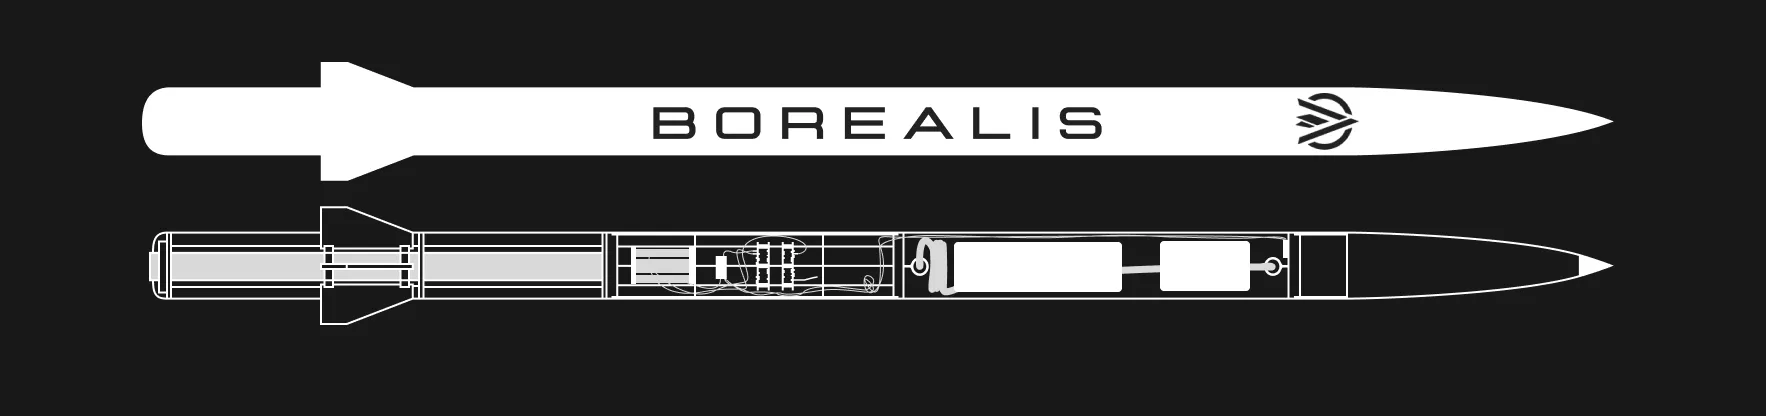
\includegraphics[width=\textwidth]{img/borealis-schema.png}
    \caption{Schema rappresentativo di \emph{Borealis}.}
    % La label ci vuole sempre e te la inventi tu: serve per riferirsi alle immagini successivamente
    \label{fig:borealis-schema}
\end{figure}

Il razzo è formato da una sezione propulsiva (\emph{Motor bay}), una fusoliera
in alluminio divisa in tre \emph{bays}:
\begin{itemize}
    \item \textbf{\emph{Electronics bay}}: contenente l'elettronica di bordo,
    \item \textbf{\emph{Payload bay}}: contenente un carico pagante sperimentale,
    \item \textbf{\emph{Parachute tube}}: contenente i due paracadute.
\end{itemize}
infine un \emph{nose cone} apribile per permettere l'espulsione del paracadute. \\

Nella \emph{Electronics bay}
è presente il computer di volo, che si occupa di
gestire il lancio e il recupero del razzo e di raccogliere dati durante il volo. \\
Il computer di volo è dotato di un sistema di telemetria che trasmette in tempo
reale i dati raccolti a una \emph{ground station}, permettendo il monitoraggio
del volo da terra.

\begin{figure}[H]
    \centering
    % Se metti solo una delle due dimensioni, l'altra scala in automatico
    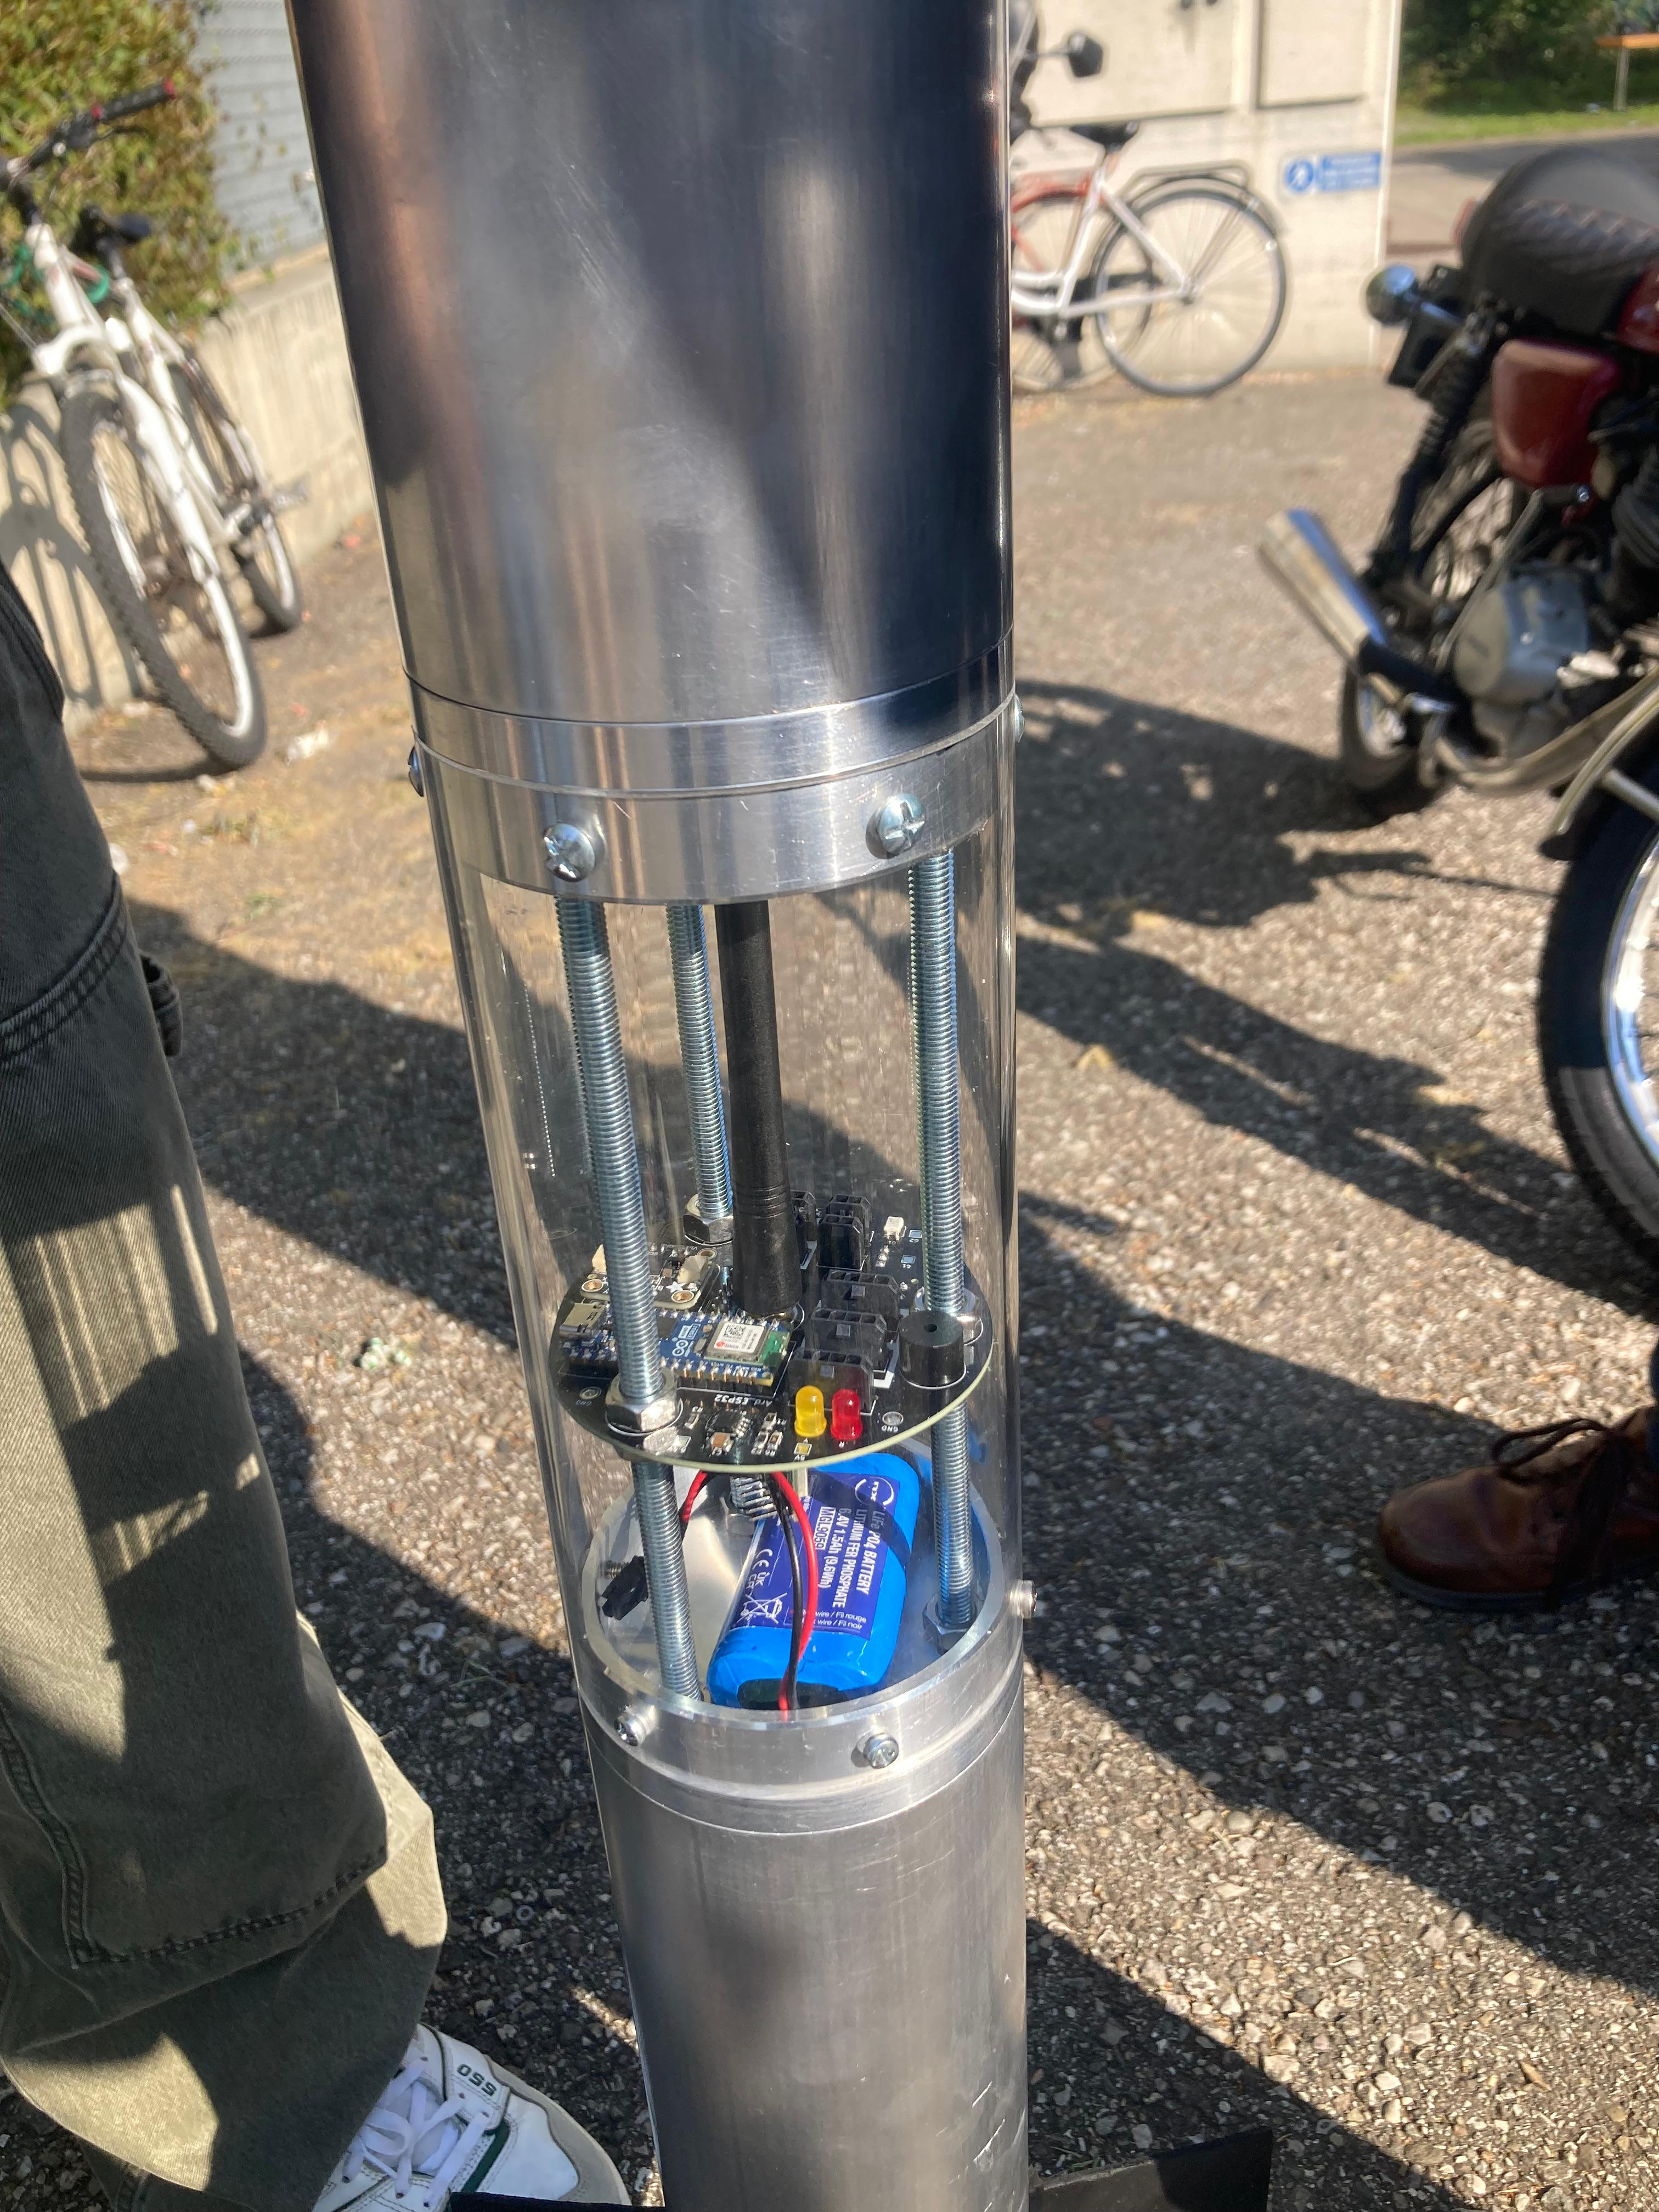
\includegraphics[width=0.5\textwidth]{img/electronics-bay.jpeg}
    \caption{\emph{Electronics bay}.}
    % La label ci vuole sempre e te la inventi tu: serve per riferirsi alle immagini successivamente
    \label{fig:electronics-bay}
\end{figure}
\sidenote{Cambiare immagine della Electronics Bay}
\section{Contesto storico della creazione e dell'impiego di razzi sperimentali}
II razzi sperimentali svolgono un ruolo cruciale nella ricerca e nello sviluppo
tecnologico sin dalla fine del XIX secolo.
Sebbene siano stati impiegati per scopi militari sin dal XIII secolo, fu tra il
1926 e il 1929 che il fisico americano Robert H. Goddard, ispirato dagli studi
di Hermann Oberth e Konstantin Tsiolkovsky sulla velocità di fuga terrestre e
sulla propulsione a razzo, realizzò il primo razzo a propellente liquido per
scopi scientifici\cite{seibert2006history}.

Da allora, i razzi sperimentali sono stati utilizzati per una vasta gamma di
applicazioni, tra cui:
\begin{itemize}
    \item La ricerca spaziale e l’esplorazione planetaria, come i razzi-sonda
          impiegati per esperimenti scientifici in microgravità.
    \item Lo studio dell’atmosfera e dei fenomeni meteorologici, come i razzi
          impiegati per analizzare la composizione degli strati superiori
          dell’atmosfera terrestre.
    \item I test di nuove tecnologie aerospaziali, inclusi materiali innovativi,
          sistemi di propulsione sperimentali, sistemi di navigazione autonoma e
          nuove tecnologie di telecomunicazione.
    \item Applicazioni educative e accademiche, che permettono a università e
          centri di ricerca di sviluppare esperimenti e formare studenti nel campo
          dell’ingegneria aerospaziale.
\end{itemize}

\section{Contesto e importanza dei sistemi di telemetria nei razzi sperimentali}
Le motivazioni per cui \`e importante sviluppare un sistema di telemetria per un
razzo sperimentale sono molteplici.

In primo luogo, il monitoraggio del volo in tempo reale permette di avere un
\emph{feedback} immediato sulle prestazioni del razzo, sulle condizioni
ambientali e sulle eventuali anomalie che possono verificarsi durante il volo.
Inoltre, la raccolta di dati durante il volo \`e fondamentale per l’analisi
post missione e per l’ottimizzazione del design del razzo.
Infine, la telemetria \`e essenziale per poter analizzare il volo in caso di
problemi o incidenti, al fine d'identificarne le cause se il sistema di
\emph{logging} a bordo dovesse andare perso.

Ciò pone delle sfide tecniche significative tra cui:
\begin{itemize}
    \item L'affidabilità della trasmissione dati, che deve essere mantenuta
          nonostante le condizioni critiche a cui il sistema è soggetto, tra cui
          accelerazioni estreme, eventi atmosferici e interferenze elettromagnetiche.
    \item L'ottimizzazione della raccolta dati, che deve avvenire in tempo reale
          e con una frequenza sufficiente per garantire la precisione delle misurazioni.
    \item La gestione del consumo energetico, che deve essere minimizzato per
          garantire l'autonomia del sistema durante il volo.
\end{itemize}

\section{Obiettivi della tesi e contributo personale}
L'obiettivo di questa tesi è la descrizione delle fasi di progettazione,
sviluppo e ottimizzazione del sistema di telemetria per il razzo Borealis di
Aurora Rocketry, offrendo una panoramica dettagliata delle tecnologie utilizzate
e delle scelte progettuali effettuate, valutando le prestazioni del sistema e
identificando possibili miglioramenti futuri.
Si vuole inoltre fornire un confronto tra le soluzioni adottate da Aurora
Rocketry e quelle utilizzate in progetti simili, al fine di valutare l'impatto
del sistema sviluppato nell'ambito della ricerca e dello sviluppo di razzi
sperimentali.

Il mio contributo personale al progetto ha riguardato tutte le fasi di sviluppo
del computer di volo, dal design iniziale alla realizzazione del prototipo, fino
alla fase di test e ottimizzazione.
Ho contribuito alla scelta delle tecnologie utilizzate, alla progettazione
dell'architettura del computer di volo e del sistema di telemetria e alla
scrittura del software per la raccolta, la strutturazione e la trasmissione dati.
Inoltre, ho partecipato attivamente alle prove sperimentali e all'analisi dei
dati raccolti, apportando modifiche e ottimizzazioni al sistema in base ai
risultati ottenuti.

\chapter{Descrizione del Computer di Volo} \label{chap:flight-computer}
\pagestyle{plain}

Il computer di volo di Borealis è basato su un microcontrollore ESP32-S3, montato
su una scheda di sviluppo Arduino Nano ESP32, un modulo di raccolta dati contenente
i sensori, e un modulo di attuatori responsabile dell'attivazione di cariche
pirotecniche tramite un circuito di innesco controllato dal microcontrollore.%
\sidenote{Inserire schema dell'architettura del computer di volo.}

I sensori utilizzati sono:
\begin{itemize}
    \item Una \ac{IMU} \emph{Bosch BNO055}\libref{lib:bno055}
          (Giroscopio, Accelerometro e Magnetometro).
    \item Due barometri \emph{Adafruit MPRLS} con presa statica \libref{lib:mprls}.
\end{itemize}
\section{Funzioni principali e componenti chiave}
Il computer di volo si occupa del monitoraggio del volo. Riceve i dati dal modulo
dei sensori, tramite algoritmi di \emph{sensor fusion} li elabora e
contemporaneamente li trasmette alla \emph{ground station}.
In particolare fa uso di un Extended Kalman Filter per filtrare e combinare i
dati ottenuti dalla \ac{IMU} e dei due barometri, ottenendo una stima
affidabile dell'orientamento, della velocità e dell'altitudine.
Il filtro mitiga gli errori dei sensori, corregge la deriva della \ac{IMU} e riduce
le incertezze delle misurazioni barometriche, combinando i dati di accelerazione,
orientamento e pressione atmosferica.

L'algoritmo di rilevamento dell'apogeo monitora l'altitudine e la velocità verticale
del razzo.
Quando la velocità verticale si annulla e il razzo inizia la discesa, il
computer di volo rileva l'apogeo e attiva la sequenza di recupero,
espellendo prima il paracadute \emph{drogue} per stabilizzare il razzo, e poi
il paracadute principale per garantire una discesa controllata.

\section{Integrazione e ruolo del sistema di telemetria}
Per la telemetria è stato impiegato un modulo \ac{LoRa} \emph{EByte E220-900T22D}
a 868MHz collegato al microcontrollore tramite un'interfaccia \ac{UART}
trasmettendo in tempo reale i dati di volo alla ground station.

Il sistema di telemetria è stato integrato nel computer di volo per permettere il
monitoraggio del volo in tempo reale e la raccolta dati durante la missione,
fornendo un'interfaccia di comunicazione tra il razzo e la \emph{ground station}.
Il sistema di telemetria è stato progettato per garantire l'affidabilità della
trasmissione dati, la precisione delle misurazioni e l'ottimizzazione del consumo
energetico.%
\sidenote{Inserire schema della comunicazione tra il computer di volo e la ground station.}
Il software di gestione della telemetria è stato sviluppato in C++17 utilizzando
una libreria open-source\libref{lib:lora} per l'interfaccia con il modulo \ac{LoRa}
e un protocollo di comunicazione personalizzato per la trasmissione e la
ricezione dei dati.

\chapter{Tecnologia \texorpdfstring{LoRa\textsuperscript{\textcopyright}}{} e la sua Applicazione} \label{chap:lora}

\section{Panoramica della tecnologia \texorpdfstring{LoRa\textsuperscript{\textcopyright}}{}}
\ac{LoRa} è una tecnologia proprietaria per la trasmissione wireless di dati a
lungo raggio e basso consumo energetico. Impiega la modulazione \ac{CSS},
che garantisce un'elevata robustezza alle interferenze e consente comunicazioni
su lunghe distanze a basso consumo energetico, a costo di una ridotta velocità di trasmissione,
che rimane comunque adeguata per applicazioni di telemetria e monitoraggio
in tempo reale. \\
\ac{LoRa} opera all'interno delle bande di frequenza \ac{ISM} non licenziate,
con specifiche allocazioni in base alla regione geografica:
\begin{itemize}
    \item \textbf{868 MHz} in Europa.
    \item \textbf{915 MHz} in Nord America.
    \item \textbf{433 MHz} in alcune aree dell’Asia.
\end{itemize}

Questa tecnologia può essere utilizzata sia in modalità \emph{point-to-point},
per la comunicazione diretta tra dispositivi, sia in un’architettura di rete più
estesa. In quest'ultimo caso, è comunemente adottata all'interno di
un'infrastruttura \ac{LoRaWAN}, che consente la trasmissione di dati a lunga
distanza tramite una rete di gateway interconnessi a server centralizzati.

\subsection{Modulazione \emph{Chirp Spread Spectrum}}
La modulazione \ac{CSS} è una tecnica di modulazione che fa uso di segnali a
\emph{chirp} per rappresentare informazioni digitali. I \emph{chirp} sono segnali
la cui frequenza varia linearmente nel tempo: quando la frequenza cresce si parla
di \emph{up-chirp}, mentre quando decresce si parla di \emph{down-chirp}.

\begin{figure}[H]
    \centering
    % Se metti solo una delle due dimensioni, l'altra scala in automatico
    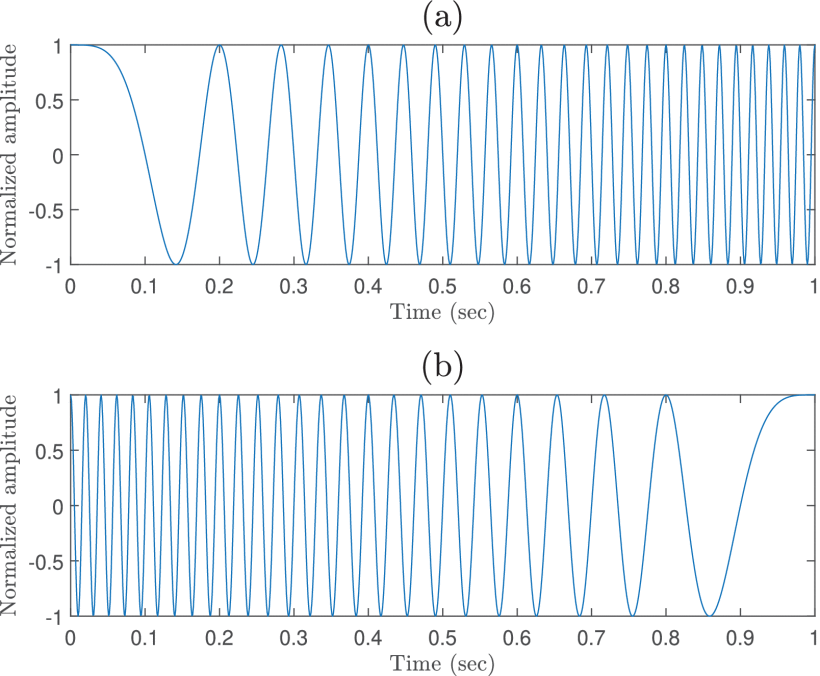
\includegraphics[width=0.75\textwidth]{img/up-chirp-down-chirp.png}
    \caption[Up-chirp e down-chirp]{%
        Esempio temporale di un \emph{up-chirp} (a) e di un \emph{down-chirp} (b).
        \textit{\tiny{Immagine adattata da \cite{10609524}.}}%
    }
    % La label ci vuole sempre e te la inventi tu: serve per riferirsi alle immagini successivamente
    \label{fig:up-chirp-down-chirp}
\end{figure}

In un sistema CSS, ogni simbolo viene rappresentato da un singolo \emph{chirp} e
la quantità di bit che esso trasporta è determinata dallo \ac{SF}, secondo la relazione
$M = 2^{SF}$, dove $M$ rappresenta il numero di simboli ortogonali (cioè distinti
tra loro).

La modulazione \ac{CSS} si basa sulla generazione di un insieme di \emph{chirp}
ortogonali ottenuti mediante traslazioni circolari nel tempo di un \emph{chirp}
di riferimento (detto \emph{chirp base}). La posizione temporale del \emph{chirp}
traslato è proporzionale al valore numerico del simbolo da trasmettere, permettendo
la generazione di $M$ forme d'onda tra loro ortogonali.

Questa proprietà consente al ricevitore di recuperare il simbolo trasmesso mediante
correlazione con i \emph{chirp} possibili, tipicamente implementata in maniera efficiente
tramite la trasformata di Fourier (FFT), rendendo il sistema robusto a rumore,
interferenze e attenuazione multipath\cite{10609524}.

\section{Specifiche tecniche dei moduli utilizzati}

Il sistema di telemetria di Borealis impiega due moduli \ac{LoRa}
\emph{EByte E220-900T22D}, uno in trasmissione a bordo del razzo e uno in
ricezione nella \emph{Ground Station}.
Il modulo impiega la ricetrasmittente \ac{LoRa} \emph{Smart Home LLCC68} e
opera nella banda di frequenza compresa tra 850.15 MHz e 930.15 MHz.

Le specifiche tecniche principali del modulo utilizzato sono riportate nella
Tabella \ref{tab:LoRa-E220-specs}. Queste caratteristiche includono la potenza di
trasmissione massima di +22 dBm (160 mW), la sensibilità del ricevitore pari a
-129 dBm, e la configurabilità dello Spreading Factor (SF) nell'intervallo
SF5 - SF12, che influisce direttamente sulla velocità di trasmissione (da 0.3 kbps
a 62.5 kbps). Inoltre, il consumo energetico del modulo varia tra 120 mA in
trasmissione alla potenza massima e 10 mA in ricezione\dsref{ds:lora}, permettendo una gestione
efficiente delle risorse in missioni di lunga durata.

\begin{table}[H]
    \centering
    \resizebox{\textwidth}{!}{
        \begin{tabular}{|c|c|}
            \hline
            \textbf{Caratteristica}                      & \textbf{Valore}         \\ \hline
            \textbf{Banda di frequenza}                  & 850.15 MHz - 930.15 MHz \\ \hline
            \textbf{Potenza di trasmissione}             & +22 dBm (160 mW)        \\ \hline
            \textbf{Sensibilità del ricevitore}          & -129 dBm                \\ \hline
            \textbf{Spreading Factor (SF)}               & SF5 - SF12              \\ \hline
            \textbf{Velocità di trasmissione}            & 0.3 kbps - 62.5 kbps    \\ \hline
            \textbf{Consumo in trasmissione (a +22 dBm)} & 120 mA                  \\ \hline
            \textbf{Consumo in ricezione}                & 10 mA                   \\ \hline
            \textbf{Interfaccia di comunicazione}        & \ac{UART} (3.3V TTL)    \\ \hline
            \textbf{Baud rate}                           & 1200 bps - 115200 bps   \\ \hline
            \textbf{Connettore antenna}                  & SMA femmina             \\ \hline
            \textbf{Impedanza connettore}                & 50 \textohm             \\ \hline
        \end{tabular}
    }
    \caption{Caratteristiche tecniche del modulo \ac{LoRa} EByte E220-900T22D.}
    \label{tab:LoRa-E220-specs}
\end{table}

\section{Specifiche delle antenne utilizzate} \label{sec:antennas}
La scelta delle antenne per il sistema telemetrico del razzo è stata guidata da
esigenze tecniche specifiche, nonostante le opzioni disponibili fossero limitate.
Le caratteristiche fondamentali del sistema richiedevano un'antenna a bordo in
grado di garantire una copertura di radiazione uniforme su una superficie quanto
più ampia possibile. Per la \emph{ground station}, invece, è stata selezionata
un'antenna direzionale.

\subsection*{Antenna omnidirezionale (Razzo)}

Per il razzo, la soluzione ottimale si è rivelata essere un'antenna omnidirezionale 
elicoidale.
Questa scelta è praticamente obbligata a causa della variazione costante dell'orientamento
del razzo durante il volo, rendendo impraticabile l'utilizzo di antenne direzionali,
a meno di non implementare sistemi complessi di controllo dell'assetto, che
tuttavia non rientrano nell'ambito del progetto attuale.

\subsection*{Antenna direzionale (Ground Station)}

Per la \emph{ground station}, è stata selezionata un'antenna direzionale. Le due
tecnologie principali prese in considerazione sono state:
\begin{itemize}
    \item Antenna Yagi
    \item Antenna Log-Periodica
\end{itemize}

La differenza principale tra questi due tipi di antenne riguarda la direzionalità.
L'antenna Log-Periodica offre una direzionalità maggiore rispetto alla Yagi,
caratteristica che, in linea di principio, sarebbe desiderabile per il sistema
di terra, in quanto consente di concentrare l'energia di ricezione in un angolo
ristretto, aumentando il guadagno e riducendo il rumore di fondo.
Tuttavia, l'eccessiva direzionalità della Log-Periodica avrebbe introdotto
delle complicazioni operative. Poiché il tracciamento del razzo durante il volo
sarà eseguito manualmente, una direzionalità troppo elevata avrebbe richiesto
una precisione di puntamento molto elevata, difficile da mantenere senza
strumenti automatizzati, aumentando il rischio di perdita temporanea del segnale.

L'antenna Yagi, con la sua direzionalità moderata, si è rivelata una scelta più
equilibrata. Essa offre un buon compromesso tra guadagno e facilità di puntamento,
consentendo un tracciamento sufficientemente preciso del razzo senza la necessità
di strumenti avanzati d'inseguimento automatico.

\subsection*{Dettagli tecnici delle antenne}

\begin{table}[H]
    \centering
    \resizebox{\textwidth}{!}{
        \begin{tabular}{|c|c|c|}
            \hline
                                & \textbf{Antenna Omnidirezionale} & \textbf{Antenna Yagi}   \\ \hline
            Marca e modello     & \emph{Siretta Delta 5A}          & \emph{Siretta Oscar 3A} \\ \hline
            Tipo                & Omnidirezionale elicoidale       & Direzionale Yagi        \\ \hline
            Frequenza di lavoro & 433 MHz - 5.9 GHz                & 850 MHz - 930 MHz       \\ \hline
            Guadagno            & 3 dBi                            & 10.55 dBi               \\ \hline
            %Direzionalità       & Bassa                            & Alta                    \\ \hline
            Angolo di copertura & 360\textdegree                   & 60\textdegree           \\ \hline
            Impedenza           & 50 \textohm                      & 50 \textohm             \\ \hline
            Polarizzazione      & Verticale                        & Verticale               \\ \hline
            Tipo di connettore  & SMA maschio                      & FME maschio             \\ \hline
            % Peso                & 28 g                             & 210 g                   \\ \hline
        \end{tabular}
    }
    \caption{Specifiche tecniche dell'antenna omnidirezionale e dell'antenna Yagi.}
    \label{tab:antenne_confronto}
\end{table}

\begin{figure}[H]
    \centering
    % Se metti solo una delle due dimensioni, l'altra scala in automatico
    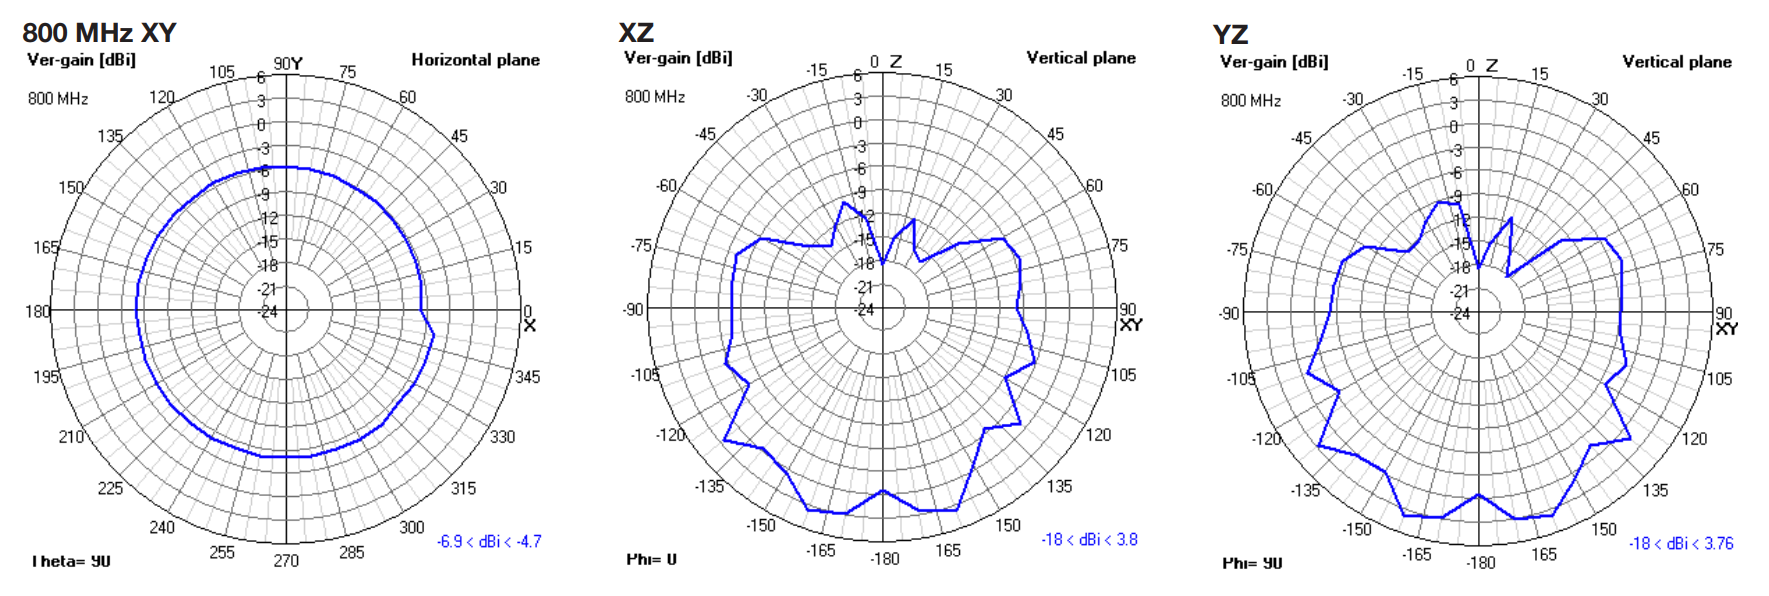
\includegraphics[width=\textwidth]{img/omnidirezionale-rad-plot.png}
    \caption[Grafici di radiazione antenna omnidirezionale]%
    {Grafici di radiazione dell'antenna omnidirezionale. \tiny{Immagine adattata da \dsref{ds:omni}}}%
    % La label ci vuole sempre e te la inventi tu: serve per riferirsi alle immagini successivamente
    \label{fig:omni-rad-plot}
\end{figure}

\begin{figure}[H]
    \centering
    % Se metti solo una delle due dimensioni, l'altra scala in automatico
    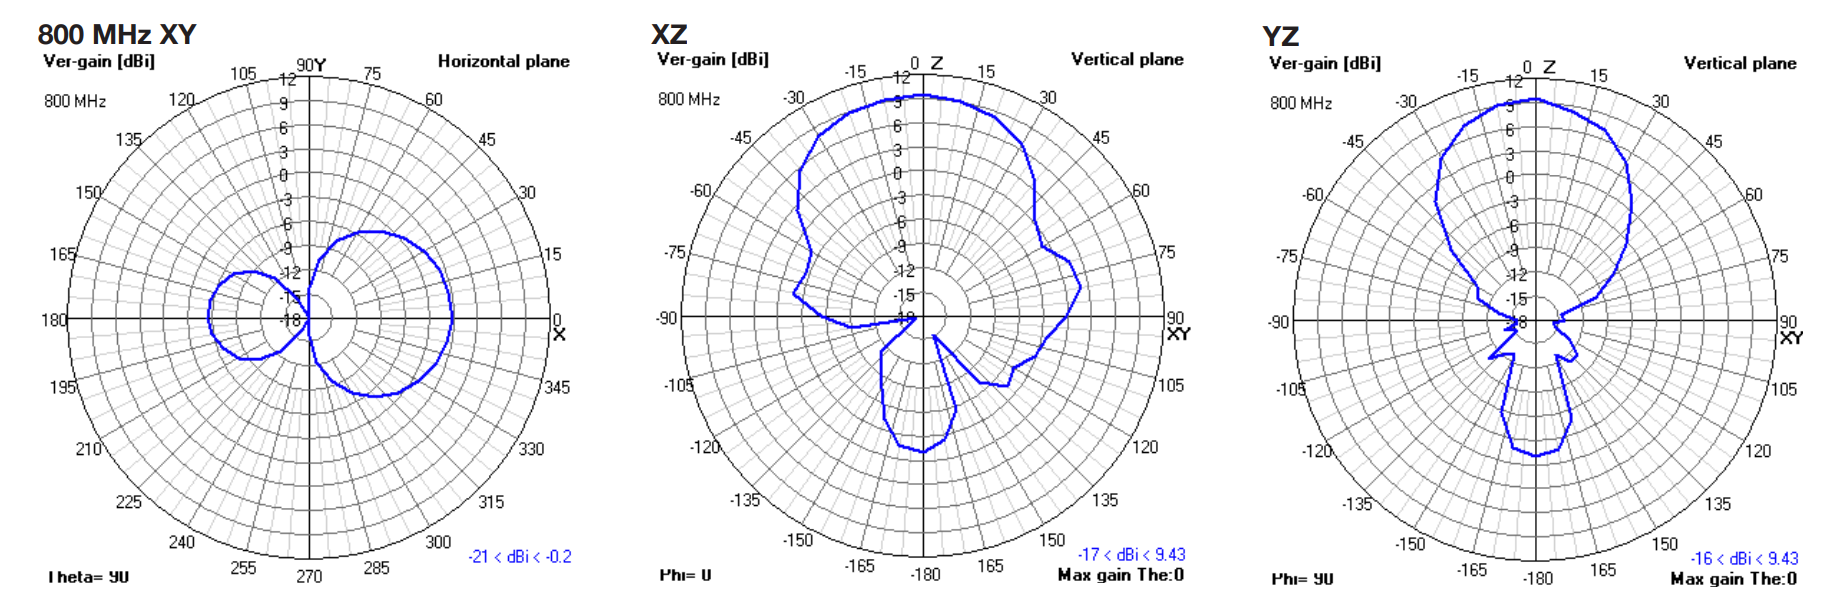
\includegraphics[width=\textwidth]{img/yagi-rad-plot.png}
    \caption[Grafici di radiazione dell'antenna Yagi]%
    {Grafici di radiazione dell'antenna Yagi. \tiny{Immagine adattata da \dsref{ds:yagi}}}%
    % La label ci vuole sempre e te la inventi tu: serve per riferirsi alle immagini successivamente
    \label{fig:yagi-rad-plot}
\end{figure}

\section{Motivazioni della scelta di \texorpdfstring{LoRa\textsuperscript{\textcopyright}}{} per il progetto}
Il progetto richiedeva di individuare una tecnologia di trasmissione dati che garantisse
un'elevata affidabilità e copertura, mantenendo un consumo energetico contenuto,
anche in un ambiente operativo complesso come quello di un razzo sperimentale.

Le caratteristiche tecniche discusse nelle sezioni precedenti rendono \ac{LoRa}
una scelta ideale per il progetto.
I test effettuati in laboratorio hanno confermato la capacità dei moduli
ricetrasmittenti impiegati di soddisfare i requisiti di trasmissione dati del
sistema di telemetria.

In letteratura sono stati documentati numerosi casi di applicazione di \ac{LoRa}
in sistemi simili\cite{Misbahuddin2022, Ma2024}, che hanno dimostrato la sua
efficacia in ambienti operativi critici, garantendo trasmissioni dati stabili e
affidabili.

Infine, l'ampia diffusione dell'uso di \ac{LoRa} nell'\ac{IoT} e la conseguente
vasta disponibilità di hardware a costi contenuti hanno reso questa tecnologia
una scelta conveniente e accessibile per il progetto.

\chapter{Implementazione del Sistema di Telemetria} \label{chap:telemetry}

% In questo capitolo verranno discussi i dettagli di progettazione e di implementazione
% del software che gestisce la telemetria a bordo di Borealis e nella \emph{ground station}.

\section{Architettura del sistema di trasmissione dati}
Il sistema di trasmissione dati impiegato su Borealis è basato su un'architettura
punto-punto monodirezionale.

Come discusso nel capitolo \ref{chap:lora} il sistema è composto dai seguenti componenti principali:
\begin{itemize}
    \item \textbf{Modulo \ac{LoRa} trasmettitore (Razzo)}: EByte E220-900T22D per
          la trasmissione della telemetria alla \emph{ground station} con antenna
          omnidirezionale (Sez. \ref{sec:antennas}).
          Collegato tramite interfaccia \ac{UART} al computer di volo.
    \item \textbf{Modulo \ac{LoRa} ricevitore (Ground Station)}: EByte E220-900T22D,
          identico al ricevente, impiegato nella \emph{ground station} per
          ricevere i dati con antenna direzionale Yagi (Sez. \ref{sec:antennas}).
          Collegato ad un microcontrollore ESP32-S3 tramite interfaccia \ac{UART}
          che si occupa di inviare i dati ricevuti ad un PC tramite connessione seriale.
\end{itemize}

Il flusso dei dati nel sistema è il seguente:
\begin{enumerate}
    \item I dati di volo vengono raccolti dai sensori a bordo del razzo e inviati al computer di volo.
    \item Il computer di volo elabora i dati attraverso un \ac{EKF} che permette di derivare l'altitudine e la velocità verticale del razzo.
    \item I dati elaborati vengono inseriti in un oggetto JSON.
    \item L'oggetto JSON viene serializzato e segmentato per rispettare i limiti di dimensione del payload dei moduli \ac{LoRa}.
    \item Ogni segmento viene inserito in un pacchetto ad-hoc per gestire la logica di trasmissione e ricezione.
    \item I dati serializzati vengono trasmessi al modulo \ac{LoRa} trasmettitore via \ac{UART}
    \item Il modulo \ac{LoRa} trasmettitore invia i pacchetti dati via wireless.
    \item Il modulo \ac{LoRa} ricevitore riceve i dati trasmessi.
    \item I dati ricevuti vengono deserializzati, ricomponendo il \emph{payload} originale.
    \item Il \emph{payload} viene inviato al PC per essere salvati e in seguito analizzati.
\end{enumerate} \sidenote{Usa uno schema a blocchi per rappresentarlo}

Vista la presenza di forti vibrazioni, accelerazioni estreme,
variazioni continue di assetto e orientamento, condizioni atmosferiche variabili
e possibili interferenze elettromagnetiche, sono stati valutati
gli impatti che questi fattori possono avere sulla trasmissione dei dati e sulla
loro integrità. \\
Abbiamo calcolato che la banda di frequenza di 868 MHz, utilizzata dai moduli
\ac{LoRa} impiegati, non è soggetta a interferenze significative da parte di altri 
dispositivi e che la modulazione \ac{CSS} impiegata garantisce una robustezza 
adeguata contro le interferenze, il rumore ambientale e l'effetto Doppler, 
permettendo una trasmissione affidabile anche in condizioni difficili.
Bisogna inoltre tenere conto che nella \emph{ground station} non \'e previsto 
alcun sistema di inseguimento, quindi l'antenna direzionale Yagi deve essere puntata manualmente
verso il razzo durante il volo, per garantire una ricezione ottimale del segnale.

\section{Protocollo di comunicazione e gestione dati}

Il protocollo di comunicazione è stato progettato per garantire efficienza e
semplicità, consentendo la trasmissione di pacchetti dati strutturati e adattabili
a diversi formati.

Il pacchetto generato dal nodo trasmittente è composto dalle seguenti sezioni:

\begin{itemize}
    \item \textbf{\emph{Header} fisico} (3 byte), che include:
          \begin{itemize}
              \item Byte alto dell’indirizzo del destinatario
              \item Byte basso dell’indirizzo del destinatario
              \item Identificativo del canale di trasmissione
          \end{itemize}
    \item \textbf{\emph{Payload}} (200 byte): contiene i dati applicativi da trasmettere.

    \item \textbf{\emph{Footer} opzionale} (1 byte): include il valore del \ac{RSSI},
          utilizzato per la diagnostica della qualità del link.
\end{itemize}

Considerando le limitazioni fisiche del modulo \ac{LoRa} impiegato (in particolare,
la dimensione massima dei pacchetti), il protocollo è stato esteso per supportare
la segmentazione del \emph{payload}. Quando il dato da trasmettere eccede la dimensione
massima consentita, esso viene suddiviso in sotto-segmenti detti \emph{chunk},
ciascuno trasmesso come pacchetto indipendente.

Per supportare questa funzionalità è stato introdotto un \textbf{header logico}
aggiuntivo di 11 byte, il cui schema è riportato di seguito.\

Tale header include le seguenti informazioni di controllo:

\begin{itemize}
    \item \textbf{\emph{Packet Number}}: identificatore univoco della sequenza di pacchetti riferita a una singola lettura.
    \item \textbf{\emph{Total Chunks}}: numero totale di chunk in cui è stato suddiviso il \emph{payload} originale.
    \item \textbf{\emph{Chunk Index}}: indice progressivo del chunk corrente all'interno della sequenza, utilizzato per la ricostruzione corretta del dato.
    \item \textbf{\emph{Payload Size}}: dimensione effettiva del \emph{payload} trasportato nel chunk, espressa in byte.
    \item \textbf{\emph{Timestamp}}: riferimento temporale associato all’invio del pacchetto, utile per analisi temporali e sincronizzazione.
    \item \textbf{\emph{Protocol Version}}: campo riservato per la gestione di versioni successive del protocollo, utile in ottica di retrocompatibilità.
\end{itemize} \sidenote{Inserire immagine schematica del pacchetto esteso}

\section{Implementazione software e algoritmi di gestione della trasmissione}
L'implementazione del software è stata realizzata in C++17, usando un approccio
modulare, applicando i principi \emph{SOLID} della programmazione a oggetti, e in
un'ottica di continua evoluzione.

\subsection{Architettura software}
In questa sezione verranno illustrati, tramite diagrammi UML e schemi, i moduli software
principali del computer di volo, del modulo trasmettitore e del modulo ricevitore.

\subsubsection{Computer di volo}
Il computer di volo è responsabile della raccolta e dell'elaborazione dei dati
provenienti dai sensori, della gestione della telemetria e dell'attivazione degli
attuatori per il recupero del razzo.

Il sistema è orchestrato da una macchina a stati finiti, che gestisce le diverse
fasi del volo, rappresentata nella Figura \ref{fig:flight-computer-fsm}. AS
\ifdefined\HCode
\else
    \begin{landscape}
        \fi
        \begin{figure}[H]
            \centering
            \vspace*{2cm}  % Reduce space from top
            \hspace*{-4cm}
            
\includegraphics[width=1.7\textwidth]{img/uml/fsm.png}
            \caption{Macchina a stati finiti del computer di volo.}
            \label{fig:flight-computer-fsm}
            \vspace*{-1cm}  % Reduce space at bottom
        \end{figure}
        \thispagestyle{empty}  % Remove page numbering for this page
        \ifdefined\HCode
        \else
    \end{landscape}
\fi

\newpage
Il computer di volo è composto da 4 elementi principali:
\paragraph{\textbf{Modulo di raccolta dati:}} Gestisce la lettura dei sensori.
\begin{figure}[H]
    \centering
    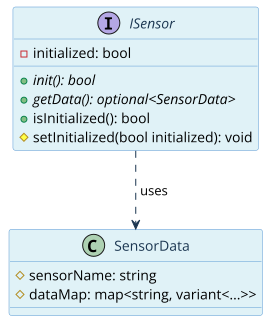
\includegraphics[width=0.5\textwidth]{img/uml/sensor.png}
    \caption{Interfaccia per la raccolta dati da un sensore.}
    \label{fig:flight-computer-data-collection}
\end{figure}

\newpage
\paragraph{\textbf{Modulo di elaborazione dati:}}Si occupa dell'elaborazione dei 
dati raccolti dai sensori, applicando un \ac{EKF} e algoritmi di \emph{sensor 
fusion} per la stime dell'altitudine e della velocità verticale, che sono 
utilizzate per il rilevamento dell'apogeo e la gestione della sequenza di recupero.
\sidenote{Inserire immagine del diagramma di flusso dell'algoritmo di elaborazione dati.}

\newpage
\paragraph{\textbf{Modulo di logging:}}Si occupa della serializzazione dei dati in formato JSON.
\begin{figure}[H]
    \centering
    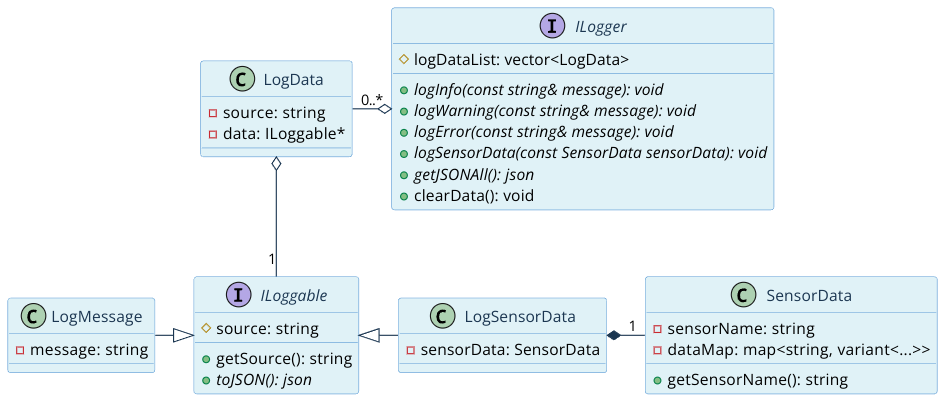
\includegraphics[width=1\textwidth]{img/uml/logger.png}
    \caption{Interfaccia per il logging dei dati.}
    \label{fig:flight-computer-logger}
\end{figure}
\newpage
\paragraph{\textbf{Modulo di telemetria:}}Si occupa della serializzazione, segmentazione
e trasmissione dei dati via \ac{LoRa}.
\begin{figure}[H]
    \centering
    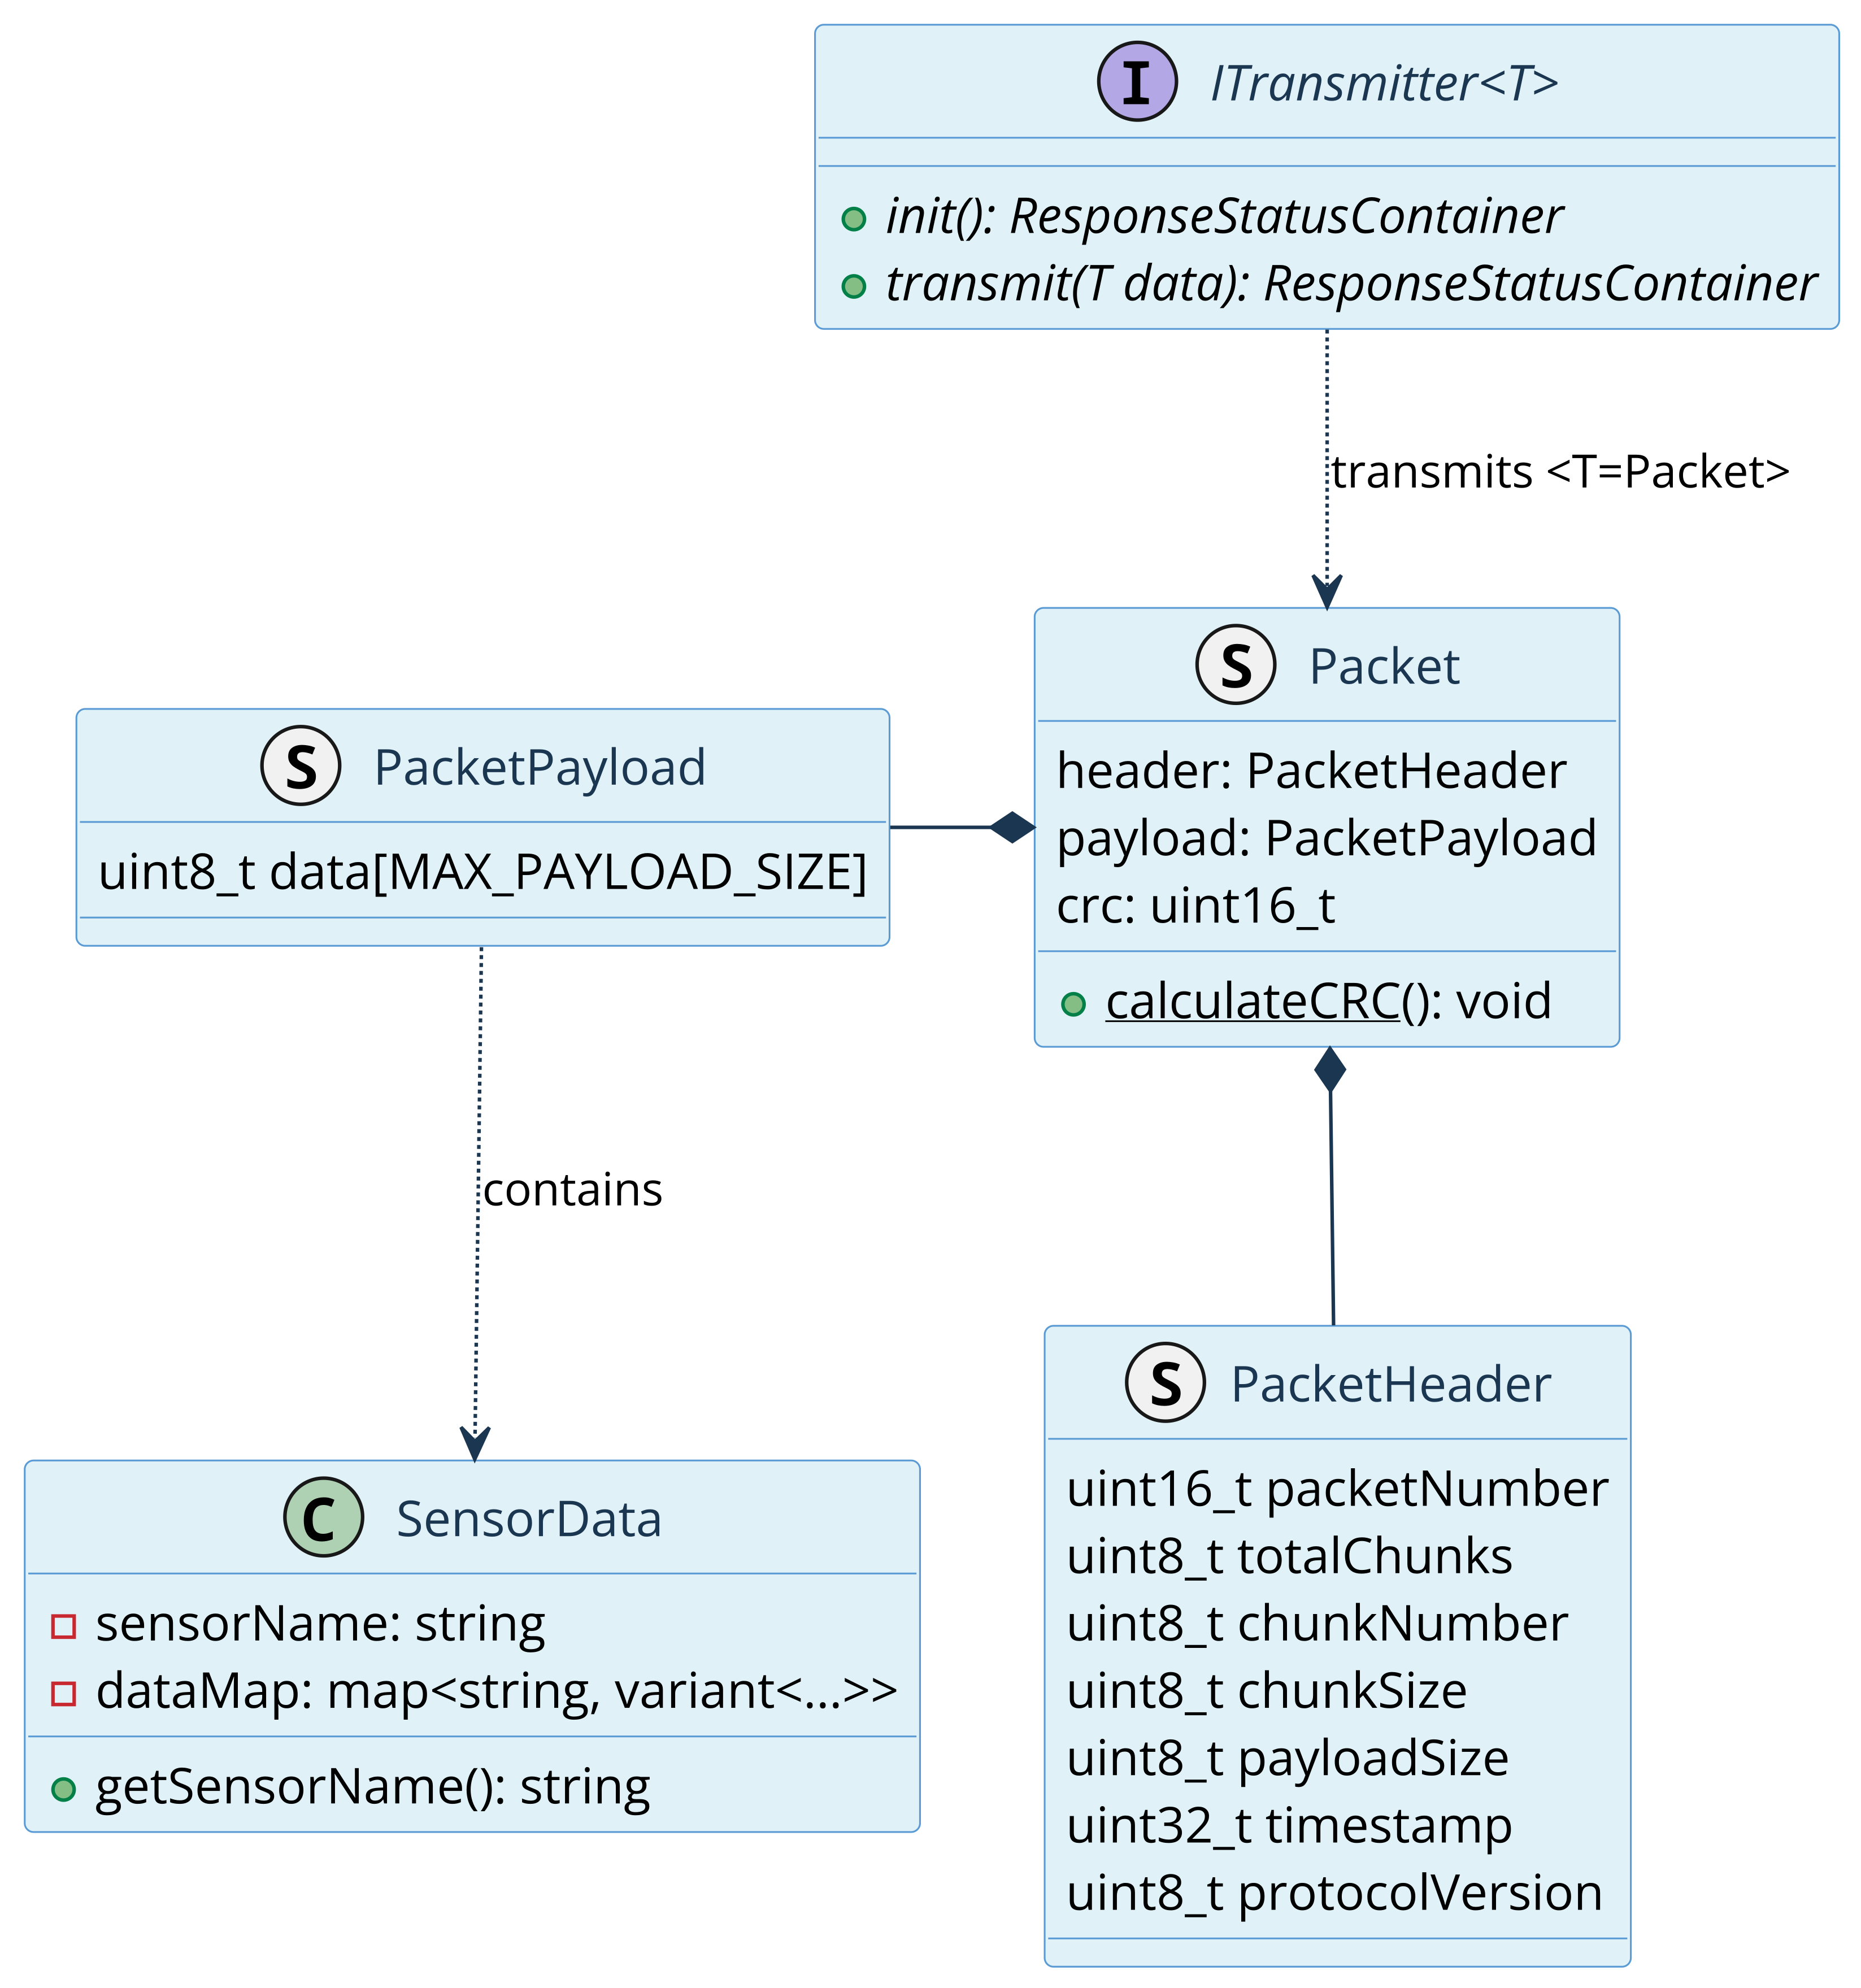
\includegraphics[width=0.8\textwidth]{img/uml/transmitter.png}
    \caption{Interfaccia per la telemetria.}
    \label{fig:flight-computer-telemetry}
\end{figure}
\newpage
\subsubsection{Ground Station}
La \emph{ground station} è responsabile della ricezione dei dati trasmessi dal
razzo, della loro deserializzazione e dell'invio al PC su cui vengono salvati.
\begin{figure}[H]
    \centering
    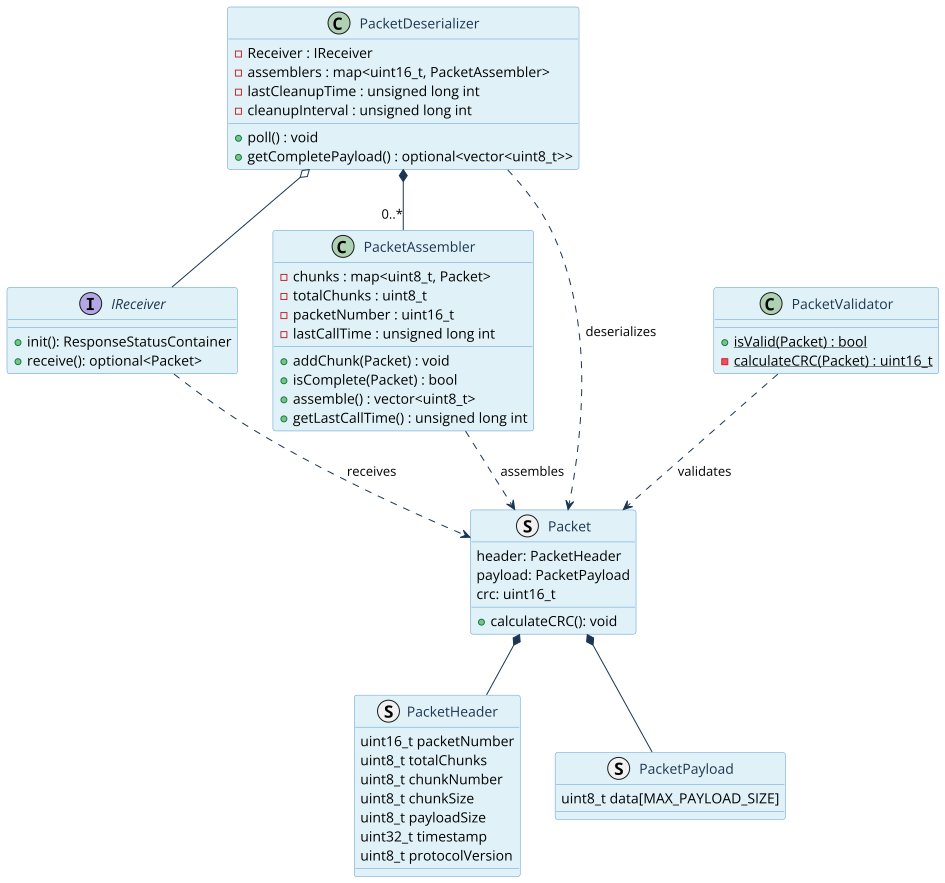
\includegraphics[width=\textwidth]{img/uml/ground-station.png}
    \caption{Architettura della \emph{ground station}.}
    \label{fig:ground-station-architecture}
\end{figure}
\newpage
\subsection{Algoritmo di ricostruzione dei dati} \sidenote{Trovare un titolo migliore}
L'algoritmo di ricostruzione del \emph{payload} originale a partire dai pacchetti 
ricevuti, permette di gestire la segmentazione dei dati e garantire l'integrità 
delle informazioni trasmesse.

L'algoritmo organizza i pacchetti ricevuti in base al loro identificativo di sequenza 
(\emph{Packet Number}), consentendo la ricostruzione dei messaggi frammentati. 
Ogni pacchetto in arrivo viene validato, verificando la consistenza dell'\emph{header} logico
e il \ac{CRC} per assicurare l'integrit\'a del contenuto.

I pacchetti validati vengono inseriti in una struttura dati temporanea, corrispondente 
alla sequenza a cui appartengono, indicizzandoli in base al \emph{Chunk Number}. 
Una volta ricevuti tutti i \emph{chunk} previsti per una sequenza, il \emph{payload} 
originale viene ricostruito, concatenando i dati dei \emph{chunk}.

Per ottimizzare l'uso delle risorse, \'e stato implementato un meccanismo di \emph{drop} 
temporizzato per le sequenze incomplete, prevenendo cos\'i l'accumulo di dati parziali, 
sfruttando la tolleranza del sistema alla perdita occasionale di letture dei dati 
dei sensori (dato il buon \emph{throughput}, verificato sperimentalmente) e la 
garanzia di disponibilità dei dati grazie al sistema di logging secondario a 
bordo del computer di volo. 
\chapter{Valutazione delle Prestazioni} \label{chap:performance}

\section{Metodologia di test e criteri di valutazione}
\section{Confronto tra simulazioni e risultati sul campo}
\section{Ottimizzazioni apportate durante lo sviluppo}

\chapter{Risultati e Analisi} \label{chap:results}

\section{Analisi dei dati raccolti durante le prove sperimentali}
\section{Limiti e possibili miglioramenti futuri}
\section{Implicazioni del sistema sviluppato per progetti simili}

\chapter{Conclusioni} \label{chap:conclusion}

\section{Riepilogo dei risultati ottenuti}
\section{Riflessioni sull'impatto del progetto nell'ambito della ricerca e dello sviluppo di razzi sperimentali}
\section{Prospettive di sviluppo futuro}

\renewcommand{\appendixtocname}{Appendici}
\renewcommand{\appendixpagename}{Appendici}
% \csname @openrightfalse\endcsname
\pagenumbering{gobble}
\begin{appendices}
    % \library{url}{name}{description}{label}
    % or
    % \library[url=...,name=...,description=...,label=...]
    % 
    % This command creates a hyperlink with a bold name and a description, 
    % and assigns a label for referencing.
    % 
    % Parameters:
    %   #1: The URL to link to.
    %   #2: The name to display in bold.
    %   #3: The description to display after the name.
    %   #4: The label for referencing.
    \newcommandx{\library}[4]{\item \href{#1}{\textbf{#2}} - #3\label{#4}}
    \renewcommand{\thechapter}{\Alph{chapter}} % Per avere "Appendice A, B, C..."
    \chapter{Librerie} \label{app:librerie}

    \begin{enumerate}
        \library{https://github.com/xreef/EByte_LoRa_E220_Series_Library}%
        {EByte LoRa E220 Series}%
        {Per la gestione dei moduli \ac{LoRa} E220.}{lib:lora}
        \library{https://github.com/adafruit/Adafruit_Sensor}%
        {Adafruit Unified Sensor}%
        {Per le API standard di gestione dei sensori.}{lib:uni-sensor}
        \library{https://github.com/adafruit/Adafruit_BNO055}%
        {Adafruit BNO055}%
        {Per la gestione della \ac{IMU}.}{lib:bno055}
        \library{https://github.com/adafruit/Adafruit_MPRLS}%
        {Adafruit MPRLS}%
        {Per la gestione dei barometri MPRLS.}{lib:mprls}
        \library{https://github.com/greiman/SdFat}%
        {Adafruit SDFat}%
        {Per la gestione del logging su scheda SD.}{lib:sdfat}
        \library{https://github.com/nlohmann/json}%
        {nlohmann-json}%
        {Per la gestione di oggetti JSON in C++.}{lib:json}
    \end{enumerate}
    \chapter{Datasheet} \label{app:datasheet}
    \begin{enumerate}
        \library{https://www.cdebyte.com/pdf-down.aspx?id=3552}%
        {Datasheet EByte E220-900T22D}%
        {Datasheet del modulo EByte E220-900T22D.}{ds:lora}
        \library{https://www.mouser.it/datasheet/2/1161/Delta_5A_Datasheet_Rev_2_2-2486634.pdf}%
        {Datasheet Siretta Delta 5A}%
        {Datasheet dell'antenna omnidirezionale Siretta Delta 5A.}{ds:omni}
        \library{https://www.siretta.com/?sdm_process_download=1&download_id=3401}%
        {Datasheet Siretta Oscar 3A}%
        {Datasheet dell'antenna Yagi Siretta Oscar 3A.}{ds:yagi}
    \end{enumerate}
    % \chapter{Embed di interi PDF}
    % \label{Appendice:C}
    % Se ti serve puoi fare embed di PDF interi con pdfpage, scegliendo anche le pagine (o mettendo - se le vuoi tutte):

    % 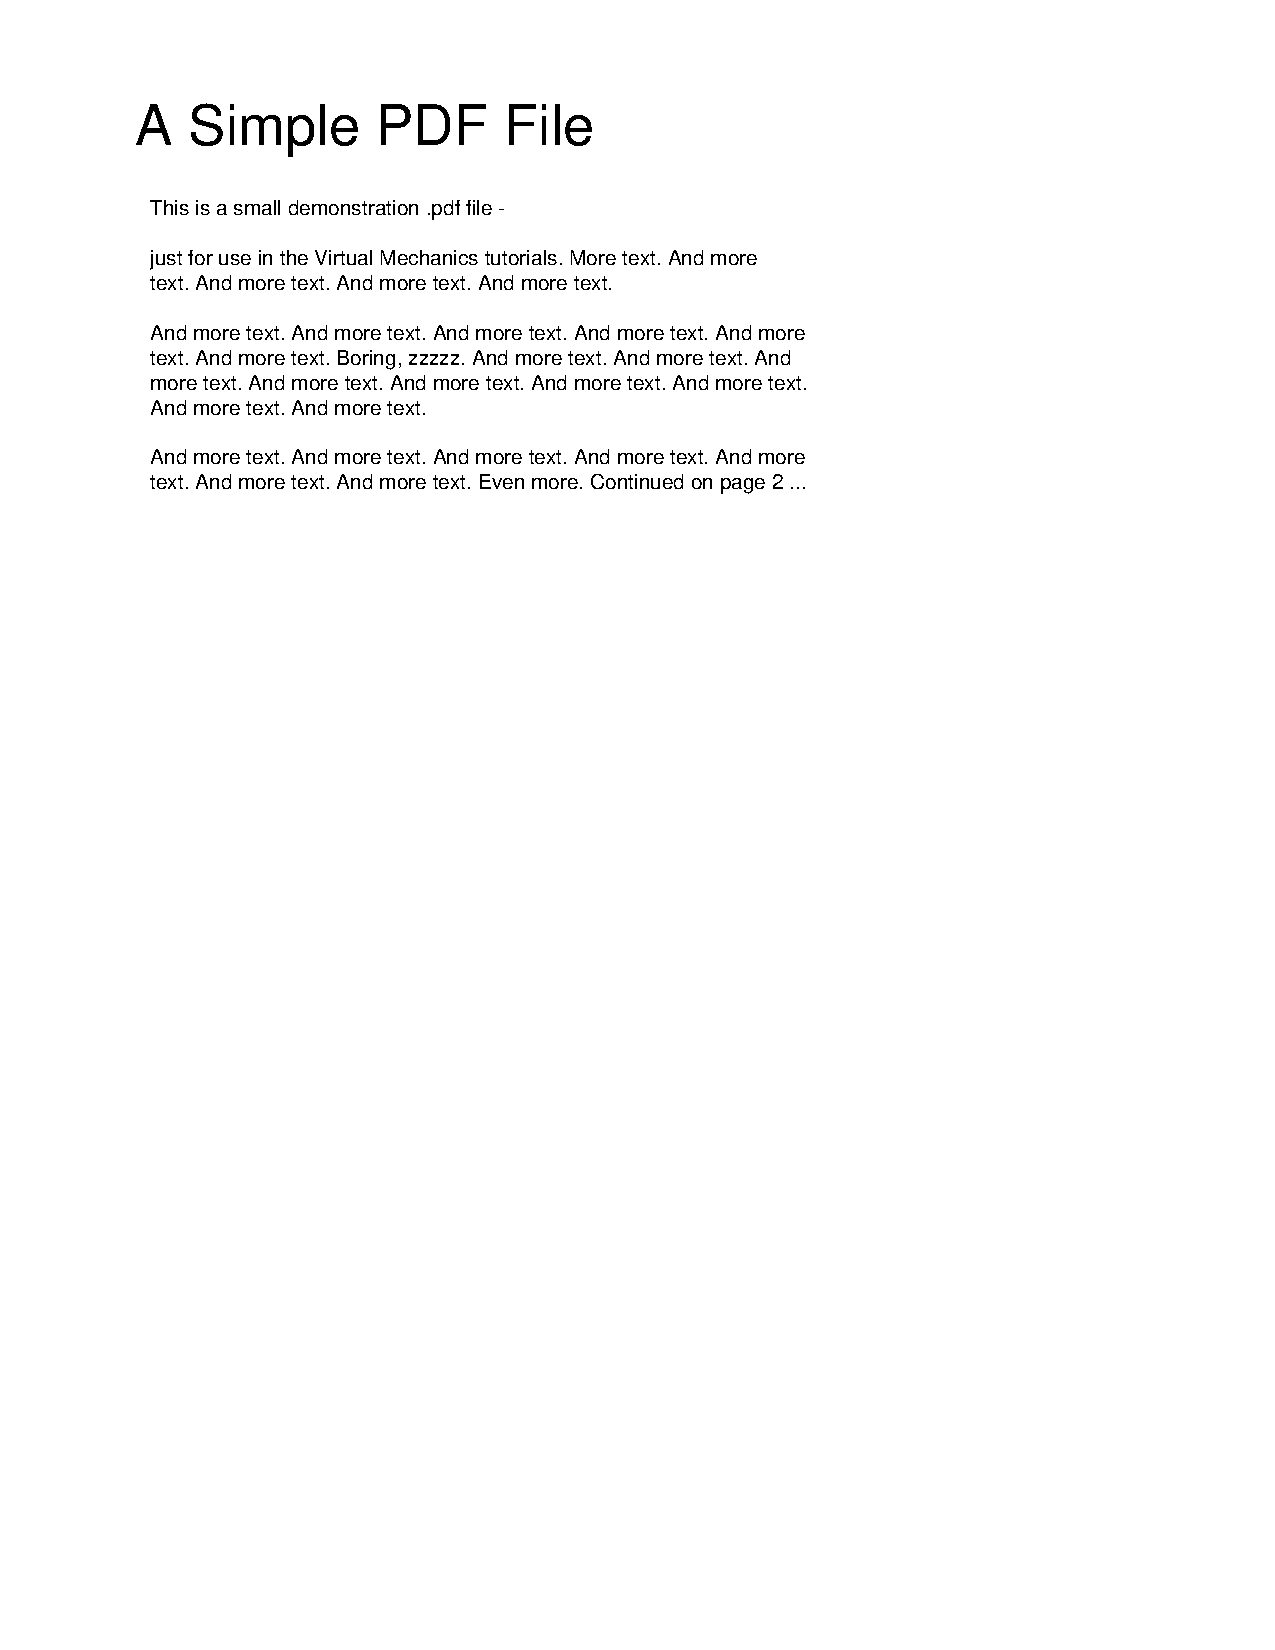
\includepdf[pages=1]{pdf/sample.pdf}
\end{appendices}
% \section{elenchi}
% \subsection{Elenchi puntati}
% \begin{itemize}
%     \item bla
%     \begin{itemize}
%         \item sub-bla
%     \end{itemize}
%     \item bla
% \end{itemize}

% \subsection{Elenchi numerati}
% \begin{enumerate}
%     \item bla1
%     \begin{enumerate}
%         \item sub bla 1
%         \item sub bla 2
%     \end{enumerate}
%     \item bla 2
% \end{enumerate}

% \subsection{Mix}
% \begin{itemize}
%     \item bla
%     \begin{enumerate}
%         \item sub bla 1
%     \end{enumerate}
%     \item bla
% \end{itemize}

% \begin{enumerate}
%     \item bla 1
%     \begin{itemize}
%         \item sub bla
%     \end{itemize}
%     \item bla 2
% \end{enumerate}

% \section{Font}
% \textbf{bla bla bla}\\
% \textit{Ancora bla bla bla}\\
% \texttt{bla bla ma in un'altra riga}

% \subsection{Sottosezione 1 - parskip}
% Grazie al package parskip se vai a capo nel .tex lasciando una riga

% ti mette un po' di spazio anche nel pdf.\\
% Attenzione però che ogni tanto questa feature fa lasciare troppo spazio tra testo e immagini / tabelle, se capita prova a togliere un po' di righe vuote. \\
% Senza questo pacchetto, una doppia new line (\texttt{$\backslash n\backslash n$}) crea un nuovo paragrafo, la cui prima riga viene leggermente indentata (un comportamento indesiderato se vieni da altri strumenti di stesura). Eventualmente, si può usare per allungare di qualche pagina alla tesi, evitando di abusarne.
% \subsection{Sottosezione 2 - capitoli}
% I capitoli iniziano sempre in una pagina dispari, quindi a volte vedrai delle pagine bianche tra uno e l'altro
% \subsubsection{Sottosottosezione 1} \label{subsub:bla}
% bla bla bla

% \chapter{Dopo l'introduzione}
% qua scrivi qualcosa
% \section{Immagini}
% Quando fai begin figure, ricordati di mettere tra quadre un modificatore di posizione: H significa esattamente nel punto dove si trova l'immagine nel file .tex e ti consiglio di usare quello, se no ci sono ad esempio t (top) e b (bottom).

% \begin{figure}[H]
%     \centering
%     % Se metti solo una delle due dimensioni, l'altra scala in automatico
%     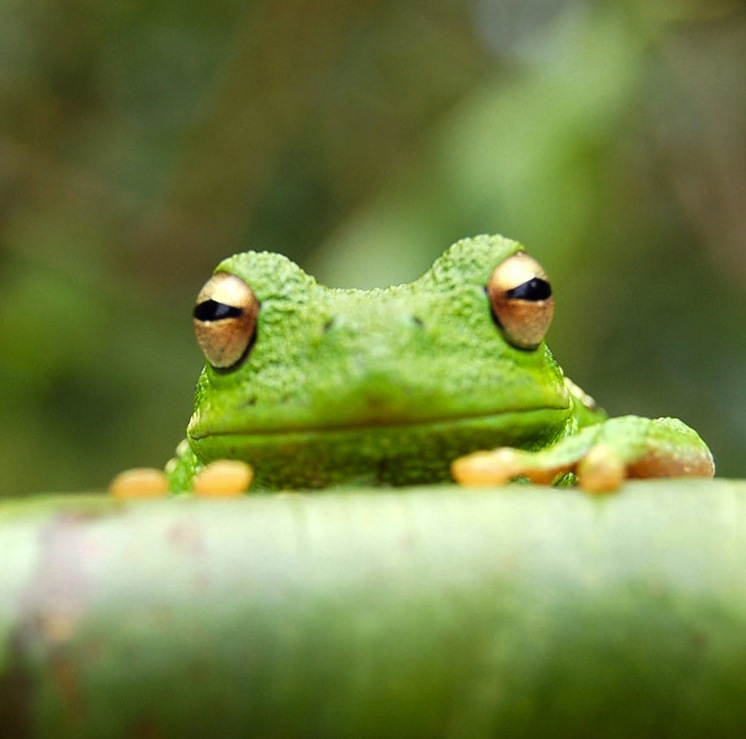
\includegraphics[height = 6cm, width=8cm]{img/frog.jpg}
%     \caption{Caption (questo viene scritto nell'indice delle figure)}
%     % La label ci vuole sempre e te la inventi tu: serve per riferirsi alle immagini successivamente
%     \label{fig:frog}
% \end{figure}

% \section{tabelle}
% \subsection{Tabella semplice}
% Anche qui nota H tra quadre, la caption e la label

% \begin{table}[H]
%     \centering
%     \begin{tabular}{|c|c|}
%     \hline
%         \textbf{Pratiche agili} & \textbf{Studenti}  \\ \hline
%         Sprint planning & 73  \\ \hline
%         Pair programming & 73  \\ \hline
%         Retrospettiva & 48  \\ \hline
%     \end{tabular}
%     \caption{Tabella semplice (anche questo scritto nell'indice delle tabelle)}
%     \label{tab:simple}
% \end{table}

% \subsection{tabelle avanzate}
% Con multirow (e multicolumn che però serve meno) puoi fare righe (colonne) più grandi del normale.\\
% \begin{table}[H]
%     \centering
%     \begin{tabular}{|c|c|c|c|c|}
%     \hline
%         \textbf{Team} & \textbf{LoC verificate} & \textbf{LoC sviluppatori} & \textbf{Ore sviluppatori} & \textbf{LoC/h}  \\ \hline
%         \multirow{2}*{1} & 1148& m: 888& m: 40& 22\cr & Diff: -1852& $\sigma$: 371& $\sigma$: 27& \\ \hline
%         \multirow{2}*{2}&1858& m: 1404& m: 65& 22\cr &  Diff: -448& $\sigma$: 1222& $\sigma$: 78& \\ \hline
%         \multirow{2}*{3}&1640& m: 1400& m: 96& 15\cr &  Diff: -2810& $\sigma$: 1417& $\sigma$: 41& \\ \hline
%     \end{tabular}
%     \caption{CAPTION}
%     \label{tab:avanz}
% \end{table}

% \subsubsection{Tabelle girate}
% Se usi landscape la tabella viene girata (nel caso dovessi inserirne una molto grande)
% \begin{landscape}
% \begin{table}[H]
%     \centering
%     \begin{tabular}{|c|c|}
%     \hline
%         \textbf{Numero} & \textbf{\#}  \\ \hline
%         UNO & 1  \\ \hline
%         DUE & 2  \\ \hline
%         TRE & 3  \\ \hline
%     \end{tabular}
%     \caption{Tabella girata}
%     \label{tab:girata}
% \end{table}

% \end{landscape}

% \section{Grafici}
% Puoi creare grafici con tikzpicture.
% Qui c'e' un grafico con asse x e y customizzabili per ogni tipo d'utilizzo.
% Tutti i tool e tutorial necessari per creare ogni tipo di grafico puo' essere trovato qui: https://tikz.dev/

% \begin{tikzpicture}
%   % Draw x-axis
%   \draw[->] (-1,0) -- (15,0) node[right] {$x$};
%   % Draw y-axis
%   \draw[->] (0,-1) -- (0,5) node[above] {$y$};

%   % Draw grid lines (optional)
%   \foreach \x in {1,2,3,4,5,6,7,8,9,10,11,12,13,14}
%     \draw (\x,-0.1) -- (\x,0.1);
%   \foreach \y in {1,2,3,4}
%     \draw (-0.1,\y) -- (0.1,\y);

%   % Draw origin
%   \fill (0,0) circle[radius=2pt];
% \end{tikzpicture}

% \section{Import di file TeX}
% Puoi importare altri file tex per intero includendoli cosi'.
% Questo e' molto utile per mettere insieme diversi capitoli di una tesi o di un grande documento in generale.

% Questo e' il contenuto del documento imported\textunderscore document.tex


% \chapter{Altri comandi}
% bla bla
% \section{Math mode}
% Per inserire simboli matematici (e lettere greche) serve la math mode:

% Usando il simbolo del dollaro hai la math mode inline: $5 \times \alpha = 3\lambda$

% Altrimenti hai quella con le barre e le quadre \[ \frac{\sum_6^i 3i\theta}{12k^2\times 7}\]

% Infine hai quelle con begin equation (che vengono numerate):
% \begin{equation}
%     \frac{1}{2}\times A_{bcd}\times E^{fgh}
% \end{equation}

% Anche le equazioni possono avere label.
% \section{url e footnote}
% per mettere un link usa url: \url{wikipedia.it}

% per fare note a piè di pagina usa footnote\footnote{Tipo questa}

% \section{Code snippets}
% per inserire code snippets, puoi usare lstlisting

% \begin{lstlisting}[language=c]
% #include<stdio.h>

% int main(void) {
%     printf("Hello World\n");
%     return 0;
% }
% \end{lstlisting}

% \section{verbatim}
% Se ti serve scrivere codice o qualcosa per cui ti serve una formattazione specifica usa verbatim:
% \begin{verbatim}
%     Qui puoi scrivere

%     come      vuoi
%     e viene tutto

% scritto
%                     monospaziato
% \end{verbatim}
%\section{riferimenti}
% Come detto prima le label servono per riferirsi ad altre parti del testo citate precendentemente.\\
% Ti consiglio di metterle sempre almeno a figure. immagini e capitoli.

% Per riferirti a qualcosa basta fare ref seguito dal nome della label, ad esempio ``vedi capitolo \ref{chap:intro}''.\\In questo modo dal pdf cliccando sulla reference, ti porta direttamente al punto giusto.
% Altri pacchetti come \texttt{fancyref} e \texttt{cleveref} (consigliato) possono aiutare nell'automatizzare la creazione delle refrence. Usando ad esempio \texttt{\cref{chap:intro}} viene generata la dicitura corrispondete all'elemento a cui si fa riferimento, seguita dalla numerazione. Eccone un esempio: \cref{chap:intro}.
%\section{citazioni}
% Per citare si usa cite seguito dal nome dell'articolo nel file.bib, ad esempio ``come visto nell'articolo di tizio\cite{greenwade93}''.

% Se non ti piace lo stile di citazione puoi modificarlo sopra dove scrivo usepackage natbib, ma quello impostato attualmente dovrebbe andare bene.



\renewcommand{\bibsection}{}
\chapter*{Riferimenti bibliografici}
\bibliography{refs}
\newpage

\newpage~\newpage
\chapter*{Ringraziamenti}
Grazie a tutti!
\end{document}
